\documentclass[PWPL]{article}
\usepackage{PWPL}
\usepackage{tipa}
\usepackage{enumerate}
\usepackage{float}
\usepackage{graphicx}
\title{Vowel Dynamics and Social Meaning in York, Northern England}
\author{Daniel Lawrence}
\begin{document}
\maketitle
\section{Introduction}
This paper investigates the factors influencing a pair of sound changes in progress: the fronting of \textipa{/u/} and \textipa{/o/}. These changes are widely attested across varieties of English, and demonstrate striking similarities in their linguistic patterning across different dialects. Despite this apparent uniformity, there is also evidence of considerable acoustic differences in the adoption of these changes (e.g. Baranowski, 2008; Koops, 2010). The present study assesses evidence for \textipa{/o/} and \textipa{/u/} fronting in a northern variety of British English, with a particular focus on the interaction of fronting and diphthongization in \textipa{/o/}. In previous work on this variety (Haddican et al., 2014), it has been claimed that the social indexing of dynamic variation in \textipa{/o/} leads speakers to resist an internal pressure to front this vowel. In light of this proposal, the present study supplements production analyses with the results of a perceptual experiment exploring listeners' sensitivity to \textipa{/u/} and \textipa{/o/} variation as a social-indexical resource. Together, these data allow the speculative claims of previous work to be tested empirically. The questions to be answered are as follows:

\begin{enumerate}
\item{What evidence is there for ongoing \textipa{/u/} and \textipa{/o/} fronting in York speech?}
\item{How does fronting interact with dynamic properties of \textipa{/o/}?}
\item{What, if any, is the role of social indexicality in constraining these changes?}
\end{enumerate}

The data are drawn from a combined corpus of production and social data collected from the same individuals, born between 1935 and 2001. This corpus is the first of its kind to be collected for a variety of British English, and provides an unprecedented opportunity to test explicit hypotheses regarding the relationship between variability in listeners' social perceptions of a change in progress and their adoption of innovative forms in production. 

The next section of this paper will provide an overview of previous work on /u/ and /o/ fronting, highlighting the patterns of apparent uniformity reported in previous work. Section 3 will provide production data demonstrating ongoing fronting in York speech, and evaluating evidence for similar patterns of uniformity in this variety. The fourth section provides an analysis of the role of dynamic variation /o/ in constraining this change. This analysis will be used as the basis for forming predictions regarding the social evaluation of /u/ and /o/ variation, to be tested in the following section. Section 5 will describe the design of the social perception experiment, and evaluate the hypotheses formed based on the production data. Conclusions and future directions will be outlined in Section 6.

\section{Previous work on \textipa{/u/} and \textipa{/o/} fronting}

The fronting of /u/ and /o/ in English dialects is one of the most widely-attested vowel changes in sociophonetic work. The tendency for the nuclei of these vowels to be realized with a more advanced tongue position is documented across North American dialects (Hall-Lew, 2009; Fridland, 2008; Baranowski, 2008), South Africa (Mesthrie, 2010), New Zealand (Easton \& Bauer, 2000), Australia (Cox,). In British English, a similar pattern of vowel fronting is reported in RP (Bauer, 1985), Kent and Reading (Torgersen \& Kerswill, 2004) and Milton Keynes (Kerswill \& Williams, 2000). Additionally, there is some evidence of fronting in Northern varieties of British English, including Bradford (Watt \& Tillotson, 2000), Carlisle (Jensen, 2010), Nottingham (Flynn, 2012) and Manchester (Baranowski \& Turton, 2015). Aside from its remarkable prevalence across varieties of English, what is striking about this change is the remarkable patterns of uniformity which emerge when analyzing the relationship between these two vowels. The patterns of interest to the present investigation are summarized below:

\begin{enumerate}[i.]
\item{The fronting of \textipa{/u/} tends to precede the fronting of \textipa{/o/} temporally}
\item{While \textipa{/u/} fronting may occur in the absence of \textipa{/o/} fronting, \textipa{/o/} fronting rarely, if ever, occurs in the absence of \textipa{/u/} fronting.}
\item{In varieties which front both \textipa{/u/} and \textipa{/o/}, the nuclei of \textipa{/u/} tend to remain more advanced than those of \textipa{/o/}}
\end{enumerate} 

Given that, in principle, processes of language change could be motived by any number of pressures, many of which may be specific to the language variety and social context studied, it is remarkable that such patterns of uniformity emerge across a wide range of dialects. This has lead many researchers to discuss back vowel fronting as an example of an `internally-motivated' change, driven by some combination of cognitive constraints (e.g. Harrington et. al, 2008) and the relationship between phonological units in English (e.g. Fruehwald, 2013). 

In addition to work highlighting uniformity in patterns of /u/ and /o/ fronting, a small literature has also explored variation in the adoption of this change. A particulary interesting finding is that, in some varieties, fronting may result in variable dynamic patterns. For example, Koops (2010) shows that Houston speakers may front /u/ in one of two ways, which differ in their fine temporal and spectral detail. By analysing dynamic properties of the vowel, Koops (2010) reveals that vowel shifts which might be considered `shared' across varieties may actually be separate innovations. Thus, it is possible that the existing literature demonstrating extensive uniformity in /u/ and /o/ fronting has ignored patterns of variability which can only be revealed through an analysis of vowel dynamics. A theoretical question underpinning this problem regards the nature of speakers' production targets: how much dynamic variation is encoded in phonological categories, and what aspect of that knowledge is affected by processes of language change? While this paper will not address this question directly, the results provide evidence that at least some aspects of dynamic variation must be part of language knowledge, and that these aspects may be particularly relevant for social-indexical work.

The varieties of English spoken in the Urban North of England are particularly suited to exploring variation and change in vowel dynamics. Historically, Northern British varieties have maintained monophthongal mid vowels \textipa{/o/} and \textipa{/e/}, in contrast to the diphthongal variants of Southern (standard) varieties. Due to a general pattern of supralocalization and increasing mobility in the UK, urban speakers are more likely than ever to encounter Southern speakers on a regular basis. 
It is thus reasonable to expect that patterns of diphthongization in /o/ might be assigned social-indexical meaning by Northern speakers, and that this might effect the trajectory of any ongoing change in that vowel. 

[text about York]


\section{Evidence for ongoing \textipa{/u/} and \textipa{/o/} fronting in York speech}
\subsection{Data \& Measurement}
\subsection{Results}
i. Change in progress in \textipa{/u/} and \textipa{/o/}\\

\begin{figure}[H]
\centering
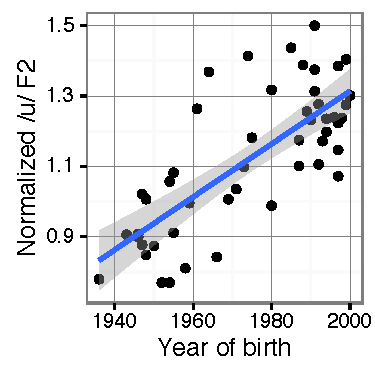
\includegraphics{uw_yob_small.pdf}
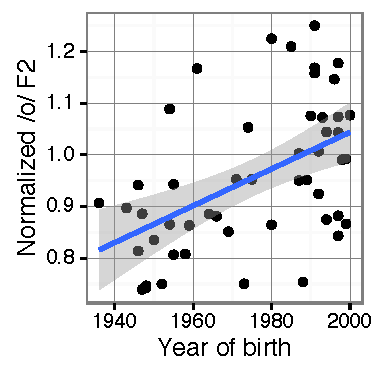
\includegraphics{ow_yob_small.pdf}
\end{figure}

ii. The relationship between \textipa{/u/} and \textipa{/o/}\\

\begin{figure}[H]
\centering
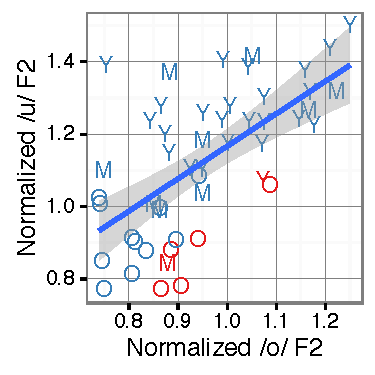
\includegraphics{ow_uw_small.pdf}
\end{figure}
\newpage
\section{The role of vowel dynamics in constraining internally-motivated change}
\subsection{Data \& Measurement}
\subsection{Results}
i. Dynamic patterns in \textipa{/u/} and \textipa{/o/}\\
ii. The relationship between fronting and diphthongization in \textipa{/o/}\\

\begin{figure}[H]
\centering
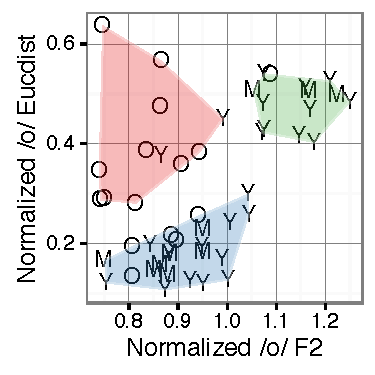
\includegraphics{ow_front_dip_small.pdf}
\end{figure}

iii. Questions to be answered\\
\section{Exploring the role of social indexicality}
\subsection{Modelling sociolinguistic perception}
\subsection{Results}
i. The social perception of \textipa{/u/}\\
ii. The social perception of \textipa{/o/}\\
\section{Conclusion}
\end{document}